% --- UPDATED RANDOMIZED QUICKSORT EXAMPLE (NEW TRACE) ---

% Step 1: Initial Array (before pivot)
\begin{frame}{Randomized Quicksort: Step 1 (Initial Array)}
  % Use columns for top-aligned split layout
  \begin{columns}[t]
    \column{0.6\textwidth}
    Consider the array:
    \[
      \renewcommand{\arraystretch}{1.5}
      \begin{array}{|c|c|c|c|c|c|c|c|}
        \hline
        15 & 3 & 1 & 10 & 9 & 0 & 6 & 4 \\
        \hline
      \end{array}
    \]
  \end{columns}
\end{frame}

\begin{frame}{Randomized Quicksort: Step 1 (Initial Array, Pivot Chosen)}
  % Use columns for top-aligned split layout
  \begin{columns}[t]
    \column{0.6\textwidth}
    Suppose the random pivot chosen is \textcolor{red}{10} (at index 3):
    \[
      \renewcommand{\arraystretch}{1.5}
      \begin{array}{|c|c|c|c|c|c|c|c|}
        \hline
        15 & 3 & 1 & \cellcolor{red!20}\textcolor{red}{10} & 9 & 0 & 6 & 4 \\
        \hline
      \end{array}
    \]
    \column{0.38\textwidth}
    \begin{minipage}[t]{\linewidth}
      \vspace{0pt}
      \begin{center}
        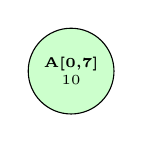
\begin{tikzpicture}[level distance=1.5cm, every node/.style={font=\tiny}]
          \node[circle, draw, fill=green!20, minimum size=1cm, align=center] (root) {
            \textbf{A[0,7]} \\
            10
          };
        \end{tikzpicture}
      \end{center}
    \end{minipage}
  \end{columns}
\end{frame}
% Step 2: Partitioning around 10
\begin{frame}{Randomized Quicksort: Step 2 (Partitioning)}
  % Use columns for top-aligned split layout
  \begin{columns}[t]
    \column{0.6\textwidth}
    After selecting pivot 10, we partition the array:
    \begin{itemize}
      \item \textcolor{green!60!black}{Left:} 4, 3, 1, 9, 0, 6 (elements before pivot position)
      \item \textcolor{red}{Middle:} 10 (pivot)
      \item \textcolor{blue}{Right:} 15 (element after pivot position)
    \end{itemize}
    After partitioning:
    \[
      \renewcommand{\arraystretch}{1.5}
      \begin{array}{|c|c|c|c|c|c|c|c|}
        \hline
        \cellcolor{green!20}\textcolor{green!60!black}{4} & \cellcolor{green!20}\textcolor{green!60!black}{3} & \cellcolor{green!20}\textcolor{green!60!black}{1} & \cellcolor{green!20}\textcolor{green!60!black}{9} & \cellcolor{green!20}\textcolor{green!60!black}{0} & \cellcolor{green!20}\textcolor{green!60!black}{6} & \cellcolor{red!20}\textcolor{red}{10} & 15 \\
        \hline
      \end{array}
    \]
    \column{0.38\textwidth}
    \begin{minipage}[t]{\linewidth}
      \vspace{0pt}
      \begin{center}
        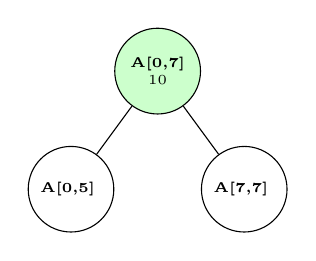
\begin{tikzpicture}[level distance=1.5cm, sibling distance=2.2cm, every node/.style={font=\tiny}]
          % Root node
          \node[circle, draw, fill=green!20, minimum size=1cm, align=center] (root) {
            \textbf{A[0,7]} \\
            10
          }
          % Left child
          child {node[circle, draw, fill=white, minimum size=1cm, align=center] {
                  \textbf{A[0,5]}
                }}
          % Right child
          child {node[circle, draw, fill=white, minimum size=1cm, align=center] {
                  \textbf{A[7,7]}
                }};
        \end{tikzpicture}
      \end{center}
    \end{minipage}
  \end{columns}
\end{frame}

% Step 3: Recurse to Left Subarray
\begin{frame}[t]{Randomized Quicksort: Step 3 (Recurse to Left Subarray)}
  % Use columns for top-aligned split layout
  \begin{columns}[t]
    \column{0.6\textwidth}
    Recurse on the left subarray:
    \\[0.5em]
    Let's choose a random pivot, say 4.
    \[
      \renewcommand{\arraystretch}{1.5}
      \begin{array}{|c|c|c|c|c|c|}
        \hline
        \cellcolor{red!20}\textcolor{red}{4} & 3 & 1 & 9 & 0 & 6 \\
        \hline
      \end{array}
    \]
    \column{0.38\textwidth}
    \begin{minipage}[t]{\linewidth}
      \vspace{0pt}
      \begin{center}
        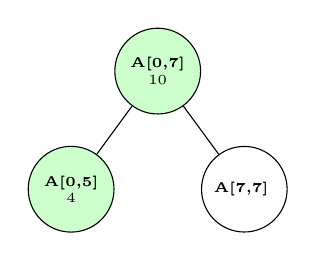
\begin{tikzpicture}[level distance=1.5cm, sibling distance=2.2cm, every node/.style={font=\tiny}]
          % Root node
          \node[circle, draw, fill=green!20, minimum size=1cm, align=center] (root) {
            \textbf{A[0,7]} \\
            10
          }
          % Left child
          child {node[circle, draw, fill=green!20, minimum size=1cm, align=center] {
                  \textbf{A[0,5]} \\
                  4
                }}
          % Right child
          child {node[circle, draw, fill=white, minimum size=1cm, align=center] {
                  \textbf{A[7,7]}
                }};
        \end{tikzpicture}
      \end{center}
    \end{minipage}
  \end{columns}
\end{frame}

% Step 3: Left Subarray [4, 3, 1, 9, 0, 6] (after pivot)
\begin{frame}[t]{Randomized Quicksort: Step 3 (Left Subarray Partitioning)}
  % Use columns for top-aligned split layout
  \begin{columns}[t]
    \column{0.6\textwidth}
    After partitioning the left subarray:
    \[
      \renewcommand{\arraystretch}{1.5}
      \begin{array}{|c|c|c|c|c|c|}
        \hline
        \cellcolor{green!20}\textcolor{green!60!black}{0} & \cellcolor{green!20}\textcolor{green!60!black}{3} & \cellcolor{green!20}\textcolor{green!60!black}{1} & \cellcolor{red!20}\textcolor{red}{4} & 9 & 6 \\
        \hline
      \end{array}
    \]
    Partition:
    \begin{itemize}
      \item \textcolor{green!60!black}{Left:} 0, 3, 1 (elements before pivot)
      \item \textcolor{red}{Middle:} 4 (pivot)
      \item \textcolor{blue}{Right:} 9, 6 (elements after pivot)
    \end{itemize}
    \column{0.38\textwidth}
    \begin{minipage}[t]{\linewidth}
      \vspace{0pt}
      \begin{center}
        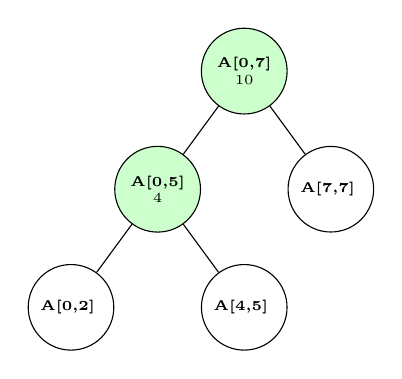
\begin{tikzpicture}[level distance=1.5cm, sibling distance=2.2cm, every node/.style={font=\tiny}]
          % Root node
          \node[circle, draw, fill=green!20, minimum size=1cm, align=center] (root) {
            \textbf{A[0,7]} \\
            10
          }
          % Left child
          % Left child
          child {node[circle, draw, fill=green!20, minimum size=1cm, align=center] {
                  \textbf{A[0,5]} \\
                  4
                }
              % New children for this step
              child {node[circle, draw, fill=white, minimum size=1cm, align=center] {
                      \textbf{A[0,2]}
                    }}
              child {node[circle, draw, fill=white, minimum size=1cm, align=center] {
                      \textbf{A[4,5]}
                    }}
            }
          % Right child
          child {node[circle, draw, fill=white, minimum size=1cm, align=center] {
                  \textbf{A[7,7]}
                }};
        \end{tikzpicture}
      \end{center}
    \end{minipage}
  \end{columns}
\end{frame}
\begin{frame}[t]{Randomized Quicksort: Step 3 (Recurse to Left Subarray)}
  % Use columns for top-aligned split layout
  \begin{columns}[t]
    \column{0.6\textwidth}
    Recurse on the left subarray:
    \\[0.5em]
    Let's choose a random pivot, say 0.
    \[
      \renewcommand{\arraystretch}{1.5}
      \begin{array}{|c|c|c|}
        \hline
        \cellcolor{red!20}\textcolor{red}{0} & 3 & 1 \\
        \hline
      \end{array}
    \]
    \column{0.38\textwidth}
    \begin{minipage}[t]{\linewidth}
      \vspace{0pt}
      \begin{center}
        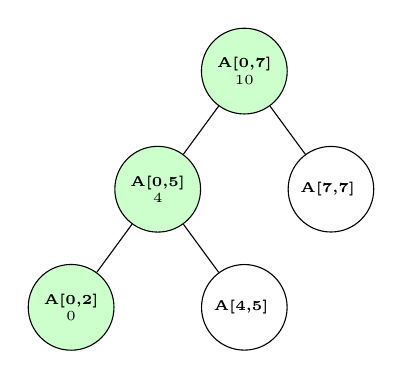
\begin{tikzpicture}[level distance=1.5cm, sibling distance=2.2cm, every node/.style={font=\tiny}]
          % Root node
          \node[circle, draw, fill=green!20, minimum size=1cm, align=center] (root) {
            \textbf{A[0,7]} \\
            10
          }
          % Left child
          % Left child
          child {node[circle, draw, fill=green!20, minimum size=1cm, align=center] {
                  \textbf{A[0,5]} \\
                  4
                }
              % New children for this step
              child {node[circle, draw, fill=green!20, minimum size=1cm, align=center] {
                      \textbf{A[0,2]}\\
                      0
                    }}
              child {node[circle, draw, fill=white, minimum size=1cm, align=center] {
                      \textbf{A[4,5]}
                    }}
            }
          % Right child
          child {node[circle, draw, fill=white, minimum size=1cm, align=center] {
                  \textbf{A[7,7]}
                }
            };
        \end{tikzpicture}
      \end{center}
    \end{minipage}
  \end{columns}
\end{frame}

% Step 3: Left Subarray [4, 3, 1, 9, 0, 6] (after pivot)
\begin{frame}[t]{Randomized Quicksort: Step 3 (Left Subarray Partitioning)}
  % Use columns for top-aligned split layout
  \begin{columns}[t]
    \column{0.6\textwidth}
    After partitioning the left subarray:
    \[
      \renewcommand{\arraystretch}{1.5}
      \begin{array}{|c|c|c|}
        \hline
        \cellcolor{red!20}\textcolor{red}{0} & 3 & 1 \\
        \hline
      \end{array}
    \]
    Partition:
    \begin{itemize}
      \item \textcolor{green!60!black}{Left:} (empty)
      \item \textcolor{red}{Middle:} 0 (pivot)
      \item \textcolor{blue}{Right:} 3, 1 (elements after pivot)
    \end{itemize}
    \column{0.38\textwidth}
    \begin{minipage}[t]{\linewidth}
      \vspace{0pt}
      \begin{center}
        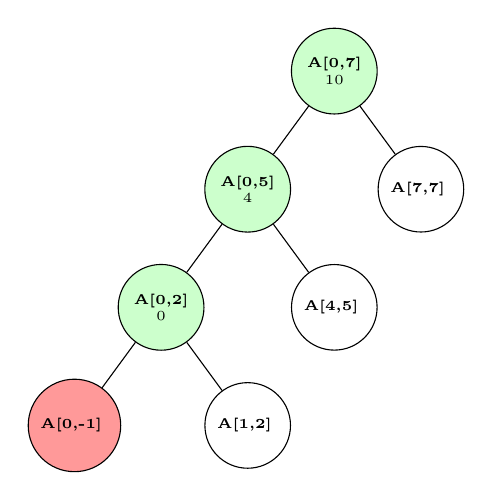
\begin{tikzpicture}[level distance=1.5cm, sibling distance=2.2cm, every node/.style={font=\tiny}]
          % Root node
          \node[circle, draw, fill=green!20, minimum size=1cm, align=center] (root) {
            \textbf{A[0,7]} \\
            10
          }
          % Left child
          % Left child
          child {node[circle, draw, fill=green!20, minimum size=1cm, align=center] {
                  \textbf{A[0,5]} \\
                  4
                }
              % New children for this step
              child {node[circle, draw, fill=green!20, minimum size=1cm, align=center] {
                      \textbf{A[0,2]}\\
                      0
                    }
                  child {node[circle, draw, fill=red!40, minimum size=1cm, align=center] {
                          \textbf{A[0,-1]}
                        }}
                  child {node[circle, draw, fill=white, minimum size=1cm, align=center] {
                          \textbf{A[1,2]}
                        }}
                }
              child {node[circle, draw, fill=white, minimum size=1cm, align=center] {
                      \textbf{A[4,5]}
                    }}
            }
          % Right child
          child {node[circle, draw, fill=white, minimum size=1cm, align=center] {
                  \textbf{A[7,7]}
                }
            };
        \end{tikzpicture}
      \end{center}
    \end{minipage}
  \end{columns}
\end{frame}

\begin{frame}[t]{Randomized Quicksort: Step 3a1 (Right of 0 Subarray)}
  % Use columns for top-aligned split layout
  \begin{columns}[t]
    \column{0.6\textwidth}
    Recurse on the right subarray:
    \\[0.5em]
    Let's choose a random pivot, say 3.
    \[
      \renewcommand{\arraystretch}{1.5}
      \begin{array}{|c|c|}
        \hline
        \cellcolor{red!20}\textcolor{red}{3} & 1 \\
        \hline
      \end{array}
    \]
    \column{0.38\textwidth}
    \begin{minipage}[t]{\linewidth}
      \vspace{0pt}
      \begin{center}
        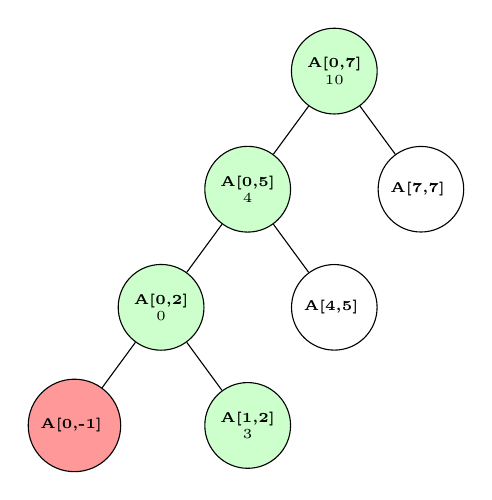
\begin{tikzpicture}[level distance=1.5cm, sibling distance=2.2cm, every node/.style={font=\tiny}]
          % Root node
          \node[circle, draw, fill=green!20, minimum size=1cm, align=center] (root) {
            \textbf{A[0,7]} \\
            10
          }
          % Left child
          % Left child
          child {node[circle, draw, fill=green!20, minimum size=1cm, align=center] {
                  \textbf{A[0,5]} \\
                  4
                }
              % New children for this step
              child {node[circle, draw, fill=green!20, minimum size=1cm, align=center] {
                      \textbf{A[0,2]}\\
                      0
                    }
                  child {node[circle, draw, fill=red!40, minimum size=1cm, align=center] {
                          \textbf{A[0,-1]}
                        }}
                  child {node[circle, draw, fill=green!20, minimum size=1cm, align=center] {
                          \textbf{A[1,2]}\\
                          3
                        }
                    }
                }
              child {node[circle, draw, fill=white, minimum size=1cm, align=center] {
                      \textbf{A[4,5]}
                    }}
            }
          % Right child
          child {node[circle, draw, fill=white, minimum size=1cm, align=center] {
                  \textbf{A[7,7]}
                }
            };
        \end{tikzpicture}
      \end{center}
    \end{minipage}
  \end{columns}
\end{frame}

% Step 3: Left Subarray [4, 3, 1, 9, 0, 6] (after pivot)
\begin{frame}[t]{Randomized Quicksort: Step 3 (Left Subarray Partitioning)}
  % Use columns for top-aligned split layout
  \begin{columns}[t]
    \column{0.6\textwidth}
    After partitioning the right subarray:
    \[
      \renewcommand{\arraystretch}{1.5}
      \begin{array}{|c|c|c|}
        \hline
        1 & \cellcolor{red!20}\textcolor{red}{3} \\
        \hline
      \end{array}
    \]
    Partition:
    \begin{itemize}
      \item \textcolor{green!60!black}{Left:} 1 (element before pivot)
      \item \textcolor{red}{Middle:} 3 (pivot)
      \item \textcolor{blue}{Right:} (empty)
    \end{itemize}
    \column{0.38\textwidth}
    \begin{minipage}[t]{\linewidth}
      \vspace{0pt} % Ensures true top alignment
      \begin{center}

        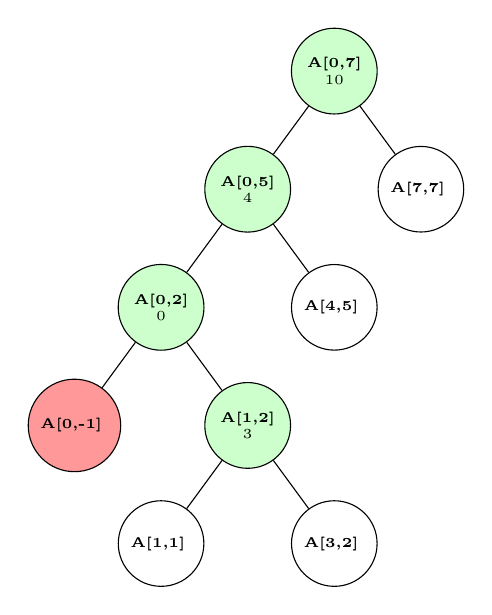
\begin{tikzpicture}[level distance=1.5cm, sibling distance=2.2cm, every node/.style={font=\tiny}]
          % Root node
          \node[circle, draw, fill=green!20, minimum size=1cm, align=center] (root) {
            \textbf{A[0,7]} \\
            10
          }
          % Left child
          child {node[circle, draw, fill=green!20, minimum size=1cm, align=center] {
                  \textbf{A[0,5]} \\
                  4
                }
              % New children for this step
              child {node[circle, draw, fill=green!20, minimum size=1cm, align=center] {
                      \textbf{A[0,2]}\\
                      0
                    }
                  child {node[circle, draw, fill=red!40, minimum size=1cm, align=center] {
                          \textbf{A[0,-1]}
                        }}
                  child {node[circle, draw, fill=green!20, minimum size=1cm, align=center] {
                          \textbf{A[1,2]}\\
                          3
                        }
                      child {node[circle, draw, fill=white, minimum size=1cm, align=center] {
                              \textbf{A[1,1]}
                            }
                        }
                      child {node[circle, draw, fill=white, minimum size=1cm, align=center] {
                              \textbf{A[3,2]}
                            }
                        }
                    }
                }
              child {node[circle, draw, fill=white, minimum size=1cm, align=center] {
                      \textbf{A[4,5]}
                    }}
            }
          % Right child
          child {node[circle, draw, fill=white, minimum size=1cm, align=center] {
                  \textbf{A[7,7]}
                }
            };
        \end{tikzpicture}
      \end{center}
    \end{minipage}
  \end{columns}
\end{frame}


% Step 3a1b: Rightmost [] (done)
\begin{frame}[t]{Randomized Quicksort: Step 3 (Left Subarray)}
  \begin{columns}[t]
    \column{0.6\textwidth}
    After partitioning the left subarray:
    \[
      \renewcommand{\arraystretch}{1.5}
      \begin{array}{|c|c|c|}
        \hline
        \cellcolor{green!20}{1} \\
        \hline
      \end{array}
    \]

    Partition:
    \begin{itemize}
      \item \textcolor{green!60!black}{Left:} (empty)
      \item \textcolor{red}{Middle:} 1 (pivot)
      \item \textcolor{blue}{Right:} (empty)
    \end{itemize}
    Single element subarray, done, return.
    \column{0.38\textwidth}
    \begin{minipage}[t]{\linewidth}
      \vspace{0pt} % Ensures true top alignment
      \begin{center}

        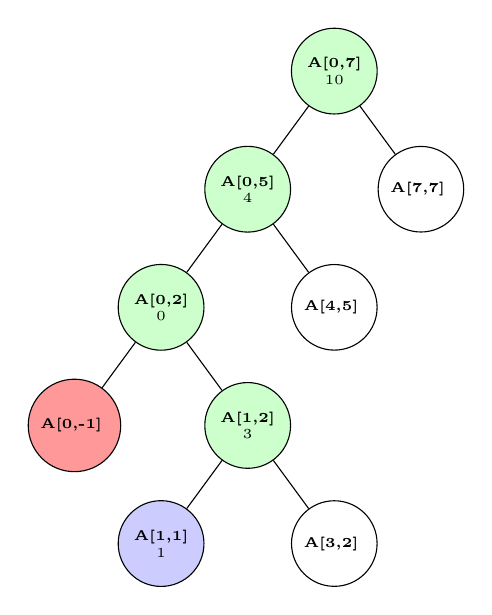
\begin{tikzpicture}[level distance=1.5cm, sibling distance=2.2cm, every node/.style={font=\tiny}]
          % Root node
          \node[circle, draw, fill=green!20, minimum size=1cm, align=center] (root) {
            \textbf{A[0,7]} \\
            10
          }
          % Left child
          child {node[circle, draw, fill=green!20, minimum size=1cm, align=center] {
                  \textbf{A[0,5]} \\
                  4
                }
              % New children for this step
              child {node[circle, draw, fill=green!20, minimum size=1cm, align=center] {
                      \textbf{A[0,2]}\\
                      0
                    }
                  child {node[circle, draw, fill=red!40, minimum size=1cm, align=center] {
                          \textbf{A[0,-1]}
                        }}
                  child {node[circle, draw, fill=green!20, minimum size=1cm, align=center] {
                          \textbf{A[1,2]}\\
                          3
                        }
                      child {node[circle, draw, fill=blue!20, minimum size=1cm, align=center] {
                              \textbf{A[1,1]}\\
                              1
                            }
                        }
                      child {node[circle, draw, fill=white, minimum size=1cm, align=center] {
                              \textbf{A[3,2]}
                            }
                        }
                    }
                }
              child {node[circle, draw, fill=white, minimum size=1cm, align=center] {
                      \textbf{A[4,5]}
                    }}
            }
          % Right child
          child {node[circle, draw, fill=white, minimum size=1cm, align=center] {
                  \textbf{A[7,7]}
                }
            };
        \end{tikzpicture}
      \end{center}
    \end{minipage}
  \end{columns}
\end{frame}

% Step 3a2: Right of 3 [] (done)
\begin{frame}{Randomized Quicksort: Step 3a2 (Right of 3 Subarray)}
  \begin{columns}[t]
    \column{0.6\textwidth}
    Recurse on the right subarray $A[3,2]$ (empty, done).
    Return to parent call $A[1,2]$
    \column{0.38\textwidth}
    \begin{minipage}[t]{\linewidth}
      \vspace{0pt} % Ensures true top alignment
      \begin{center}

        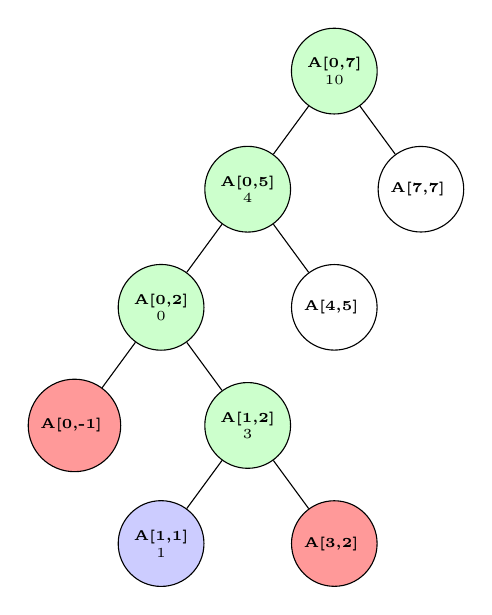
\begin{tikzpicture}[level distance=1.5cm, sibling distance=2.2cm, every node/.style={font=\tiny}]
          % Root node
          \node[circle, draw, fill=green!20, minimum size=1cm, align=center] (root) {
            \textbf{A[0,7]} \\
            10
          }
          % Left child
          child {node[circle, draw, fill=green!20, minimum size=1cm, align=center] {
                  \textbf{A[0,5]} \\
                  4
                }
              % New children for this step
              child {node[circle, draw, fill=green!20, minimum size=1cm, align=center] {
                      \textbf{A[0,2]}\\
                      0
                    }
                  child {node[circle, draw, fill=red!40, minimum size=1cm, align=center] {
                          \textbf{A[0,-1]}
                        }}
                  child {node[circle, draw, fill=green!20, minimum size=1cm, align=center] {
                          \textbf{A[1,2]}\\
                          3
                        }
                      child {node[circle, draw, fill=blue!20, minimum size=1cm, align=center] {
                              \textbf{A[1,1]}\\
                              1
                            }
                        }
                      child {node[circle, draw, fill=red!40, minimum size=1cm, align=center] {
                              \textbf{A[3,2]}
                            }
                        }
                    }
                }
              child {node[circle, draw, fill=white, minimum size=1cm, align=center] {
                      \textbf{A[4,5]}
                    }}
            }
          % Right child
          child {node[circle, draw, fill=white, minimum size=1cm, align=center] {
                  \textbf{A[7,7]}
                }
            };
        \end{tikzpicture}
      \end{center}
    \end{minipage}
  \end{columns}
\end{frame}
\begin{frame}{Randomized Quicksort: Step 3a2 (Right of 3 Subarray)}
  \begin{columns}[t]
    \column{0.6\textwidth}
    Return to parent call $A[0,2]$
    \column{0.38\textwidth}
    \begin{minipage}[t]{\linewidth}
      \vspace{0pt} % Ensures true top alignment
      \begin{center}

        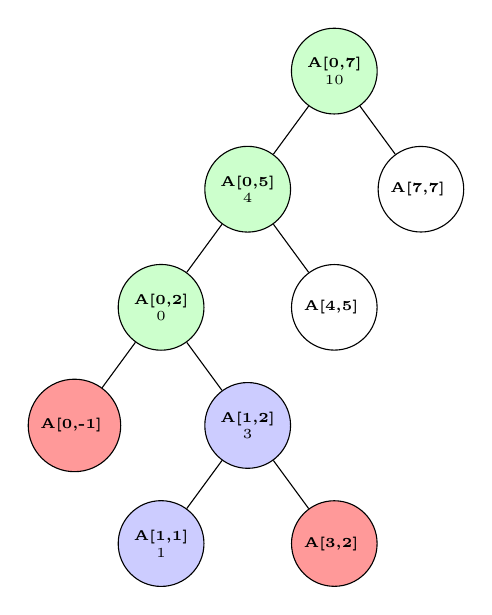
\begin{tikzpicture}[level distance=1.5cm, sibling distance=2.2cm, every node/.style={font=\tiny}]
          % Root node
          \node[circle, draw, fill=green!20, minimum size=1cm, align=center] (root) {
            \textbf{A[0,7]} \\
            10
          }
          % Left child
          child {node[circle, draw, fill=green!20, minimum size=1cm, align=center] {
                  \textbf{A[0,5]} \\
                  4
                }
              % New children for this step
              child {node[circle, draw, fill=green!20, minimum size=1cm, align=center] {
                      \textbf{A[0,2]}\\
                      0
                    }
                  child {node[circle, draw, fill=red!40, minimum size=1cm, align=center] {
                          \textbf{A[0,-1]}
                        }}
                  child {node[circle, draw, fill=blue!20, minimum size=1cm, align=center] {
                          \textbf{A[1,2]}\\
                          3
                        }
                      child {node[circle, draw, fill=blue!20, minimum size=1cm, align=center] {
                              \textbf{A[1,1]}\\
                              1
                            }
                        }
                      child {node[circle, draw, fill=red!40, minimum size=1cm, align=center] {
                              \textbf{A[3,2]}
                            }
                        }
                    }
                }
              child {node[circle, draw, fill=white, minimum size=1cm, align=center] {
                      \textbf{A[4,5]}
                    }}
            }
          % Right child
          child {node[circle, draw, fill=white, minimum size=1cm, align=center] {
                  \textbf{A[7,7]}
                }
            };
        \end{tikzpicture}
      \end{center}
    \end{minipage}
  \end{columns}
\end{frame}
\begin{frame}{Randomized Quicksort: Step 3a2 (Right of 3 Subarray)}
  \begin{columns}[t]
    % Use columns for top-aligned split layout
    \column{0.6\textwidth}
    Recurse on the right subarray $A[4,5]$:
    \\[0.5em]
    Let's choose a random pivot, say 9.
    \[
      \renewcommand{\arraystretch}{1.5}
      \begin{array}{|c|c|}
        \hline
        \cellcolor{red!20}\textcolor{red}{9} & 6 \\
        \hline
      \end{array}
    \]
    \column{0.38\textwidth}
    \begin{minipage}[t]{\linewidth}
      \vspace{0pt} % Ensures true top alignment
      \begin{center}

        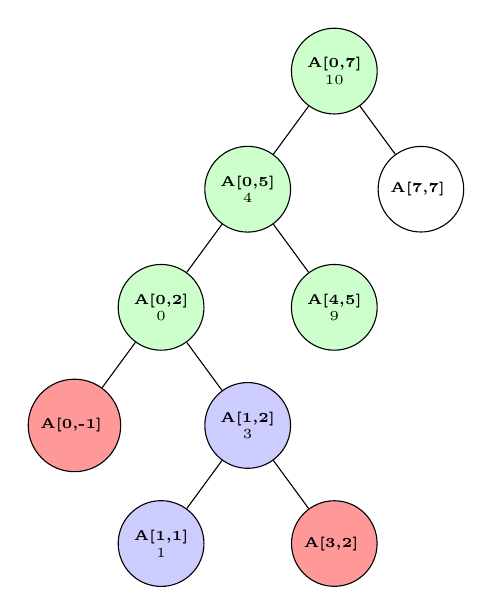
\begin{tikzpicture}[level distance=1.5cm, sibling distance=2.2cm, every node/.style={font=\tiny}]
          % Root node
          \node[circle, draw, fill=green!20, minimum size=1cm, align=center] (root) {
            \textbf{A[0,7]} \\
            10
          }
          % Left child
          child {node[circle, draw, fill=green!20, minimum size=1cm, align=center] {
                  \textbf{A[0,5]} \\
                  4
                }
              % New children for this step
              child {node[circle, draw, fill=green!20, minimum size=1cm, align=center] {
                      \textbf{A[0,2]}\\
                      0
                    }
                  child {node[circle, draw, fill=red!40, minimum size=1cm, align=center] {
                          \textbf{A[0,-1]}
                        }}
                  child {node[circle, draw, fill=blue!20, minimum size=1cm, align=center] {
                          \textbf{A[1,2]}\\
                          3
                        }
                      child {node[circle, draw, fill=blue!20, minimum size=1cm, align=center] {
                              \textbf{A[1,1]}\\
                              1
                            }
                        }
                      child {node[circle, draw, fill=red!40, minimum size=1cm, align=center] {
                              \textbf{A[3,2]}
                            }
                        }
                    }
                }
              child {node[circle, draw, fill=green!20, minimum size=1cm, align=center] {
                      \textbf{A[4,5]}\\
                      9
                    }}
            }
          % Right child
          child {node[circle, draw, fill=white, minimum size=1cm, align=center] {
                  \textbf{A[7,7]}
                }
            };
        \end{tikzpicture}
      \end{center}
    \end{minipage}
  \end{columns}
\end{frame}
% Step 3b: Right of 4 [9, 6], pivot 9
\begin{frame}{Randomized Quicksort: Step 3b (Right of 4 Subarray)}


  \begin{columns}[t]
    % Use columns for top-aligned split layout
    \column{0.6\textwidth}
    Recurse on the right subarray $A[4,5]$:
    \\[0.5em]

    Suppose the random pivot is \textcolor{red}{9}:
    \[
      \renewcommand{\arraystretch}{1.5}
      \begin{array}{|c|c|}
        \hline
        6 & \cellcolor{red!20}\textcolor{red}{9} \\
        \hline
      \end{array}
    \]

    Partition:
    \begin{itemize}
      \item \textcolor{green!60!black}{Left:} 6 (element before pivot)
      \item \textcolor{red}{Middle:} 9 (pivot)
      \item \textcolor{blue}{Right:} (empty)
    \end{itemize}
    \column{0.38\textwidth}
    \begin{minipage}[t]{\linewidth}
      \vspace{0pt} % Ensures true top alignment
      \begin{center}

        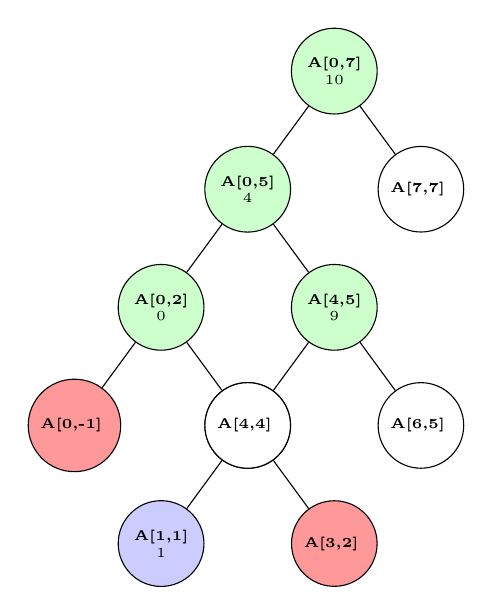
\begin{tikzpicture}[level distance=1.5cm, sibling distance=2.2cm, every node/.style={font=\tiny}]
          % Root node
          \node[circle, draw, fill=green!20, minimum size=1cm, align=center] (root) {
            \textbf{A[0,7]} \\
            10
          }
          % Left child
          child {node[circle, draw, fill=green!20, minimum size=1cm, align=center] {
                  \textbf{A[0,5]} \\
                  4
                }
              % New children for this step
              child {node[circle, draw, fill=green!20, minimum size=1cm, align=center] {
                      \textbf{A[0,2]}\\
                      0
                    }
                  child {node[circle, draw, fill=red!40, minimum size=1cm, align=center] {
                          \textbf{A[0,-1]}
                        }}
                  child {node[circle, draw, fill=blue!20, minimum size=1cm, align=center] {
                          \textbf{A[1,2]}\\
                          3
                        }
                      child {node[circle, draw, fill=blue!20, minimum size=1cm, align=center] {
                              \textbf{A[1,1]}\\
                              1
                            }
                        }
                      child {node[circle, draw, fill=red!40, minimum size=1cm, align=center] {
                              \textbf{A[3,2]}
                            }
                        }
                    }
                }
              child {node[circle, draw, fill=green!20, minimum size=1cm, align=center] {
                      \textbf{A[4,5]}\\
                      9
                    }
                  child {node[circle, draw, fill=white, minimum size=1cm, align=center] {
                          \textbf{A[4,4]}
                        }}
                  child {node[circle, draw, fill=white, minimum size=1cm, align=center] {
                          \textbf{A[6,5]}
                        }}
                }
            }
          % Right child
          child {node[circle, draw, fill=white, minimum size=1cm, align=center] {
                  \textbf{A[7,7]}
                }
            };
        \end{tikzpicture}
      \end{center}
    \end{minipage}
  \end{columns}
\end{frame}

% Step 3b1: Leftmost [6] (done)
\begin{frame}{Randomized Quicksort: Step 3b1 (Leftmost Subarray)}
  \begin{columns}[t]
    \column{0.6\textwidth}
    After partitioning the left subarray:
    \[
      \renewcommand{\arraystretch}{1.5}
      \begin{array}{|c|c|c|}
        \hline
        \cellcolor{green!20}{6} \\
        \hline
      \end{array}
    \]

    Partition:
    \begin{itemize}
      \item \textcolor{green!60!black}{Left:} (empty)
      \item \textcolor{red}{Middle:} 6 (pivot)
      \item \textcolor{blue}{Right:} (empty)
    \end{itemize}
    Single element subarray, done, return.
    \column{0.38\textwidth}
    \begin{minipage}[t]{\linewidth}
      \vspace{0pt} % Ensures true top alignment
      \begin{center}

        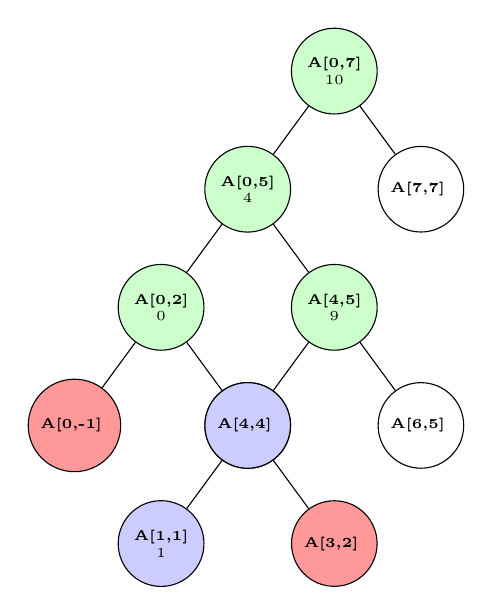
\begin{tikzpicture}[level distance=1.5cm, sibling distance=2.2cm, every node/.style={font=\tiny}]
          % Root node
          \node[circle, draw, fill=green!20, minimum size=1cm, align=center] (root) {
            \textbf{A[0,7]} \\
            10
          }
          % Left child
          child {node[circle, draw, fill=green!20, minimum size=1cm, align=center] {
                  \textbf{A[0,5]} \\
                  4
                }
              % New children for this step
              child {node[circle, draw, fill=green!20, minimum size=1cm, align=center] {
                      \textbf{A[0,2]}\\
                      0
                    }
                  child {node[circle, draw, fill=red!40, minimum size=1cm, align=center] {
                          \textbf{A[0,-1]}
                        }}
                  child {node[circle, draw, fill=blue!20, minimum size=1cm, align=center] {
                          \textbf{A[1,2]}\\
                          3
                        }
                      child {node[circle, draw, fill=blue!20, minimum size=1cm, align=center] {
                              \textbf{A[1,1]}\\
                              1
                            }
                        }
                      child {node[circle, draw, fill=red!40, minimum size=1cm, align=center] {
                              \textbf{A[3,2]}
                            }
                        }
                    }
                }
              child {node[circle, draw, fill=green!20, minimum size=1cm, align=center] {
                      \textbf{A[4,5]}\\
                      9
                    }
                  child {node[circle, draw, fill=blue!20, minimum size=1cm, align=center] {
                          \textbf{A[4,4]}
                        }}
                  child {node[circle, draw, fill=white, minimum size=1cm, align=center] {
                          \textbf{A[6,5]}
                        }}
                }
            }
          % Right child
          child {node[circle, draw, fill=white, minimum size=1cm, align=center] {
                  \textbf{A[7,7]}
                }
            };
        \end{tikzpicture}
      \end{center}
    \end{minipage}
  \end{columns}
\end{frame}

\begin{frame}{Randomized Quicksort: Step 3b1 (Leftmost Subarray)}
  \begin{columns}[t]
    \column{0.6\textwidth}
    Recurse on the right subarray $A[6,5]$ (empty, done).
    Return to parent call $A[4,5]$\\
    Return to parent call $A[0,5]$\\
    \column{0.38\textwidth}
    \begin{minipage}[t]{\linewidth}
      \vspace{0pt} % Ensures true top alignment
      \begin{center}

        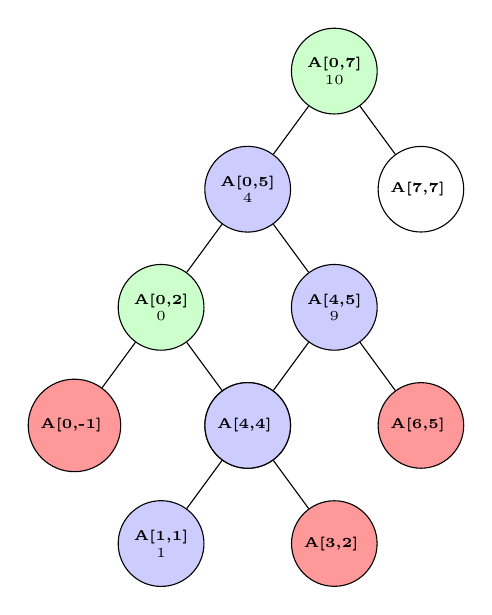
\begin{tikzpicture}[level distance=1.5cm, sibling distance=2.2cm, every node/.style={font=\tiny}]
          % Root node
          \node[circle, draw, fill=green!20, minimum size=1cm, align=center] (root) {
            \textbf{A[0,7]} \\
            10
          }
          % Left child
          child {node[circle, draw, fill=blue!20, minimum size=1cm, align=center] {
                  \textbf{A[0,5]} \\
                  4
                }
              % New children for this step
              child {node[circle, draw, fill=green!20, minimum size=1cm, align=center] {
                      \textbf{A[0,2]}\\
                      0
                    }
                  child {node[circle, draw, fill=red!40, minimum size=1cm, align=center] {
                          \textbf{A[0,-1]}
                        }}
                  child {node[circle, draw, fill=blue!20, minimum size=1cm, align=center] {
                          \textbf{A[1,2]}\\
                          3
                        }
                      child {node[circle, draw, fill=blue!20, minimum size=1cm, align=center] {
                              \textbf{A[1,1]}\\
                              1
                            }
                        }
                      child {node[circle, draw, fill=red!40, minimum size=1cm, align=center] {
                              \textbf{A[3,2]}
                            }
                        }
                    }
                }
              child {node[circle, draw, fill=blue!20, minimum size=1cm, align=center] {
                      \textbf{A[4,5]}\\
                      9
                    }
                  child {node[circle, draw, fill=blue!20, minimum size=1cm, align=center] {
                          \textbf{A[4,4]}
                        }}
                  child {node[circle, draw, fill=red!40, minimum size=1cm, align=center] {
                          \textbf{A[6,5]}
                        }}
                }
            }
          % Right child
          child {node[circle, draw, fill=white, minimum size=1cm, align=center] {
                  \textbf{A[7,7]}
                }
            };
        \end{tikzpicture}
      \end{center}
    \end{minipage}
  \end{columns}
\end{frame}
\begin{frame}{Randomized Quicksort: Step 3b1 (Leftmost Subarray)}
  \begin{columns}[t]
    \column{0.6\textwidth}
    Recurse on the right subarray $A[7,7]$
    After partitioning the right subarray:
    \[
      \renewcommand{\arraystretch}{1.5}
      \begin{array}{|c|c|c|}
        \hline
        \cellcolor{green!20}{1} \\
        \hline
      \end{array}
    \]

    Partition:
    \begin{itemize}
      \item \textcolor{green!60!black}{Left:} (empty)
      \item \textcolor{red}{Middle:} 1 (pivot)
      \item \textcolor{blue}{Right:} (empty)
    \end{itemize}
    Single element subarray, done, return.
    \column{0.38\textwidth}
    \begin{minipage}[t]{\linewidth}
      \vspace{0pt} % Ensures true top alignment
      \begin{center}

        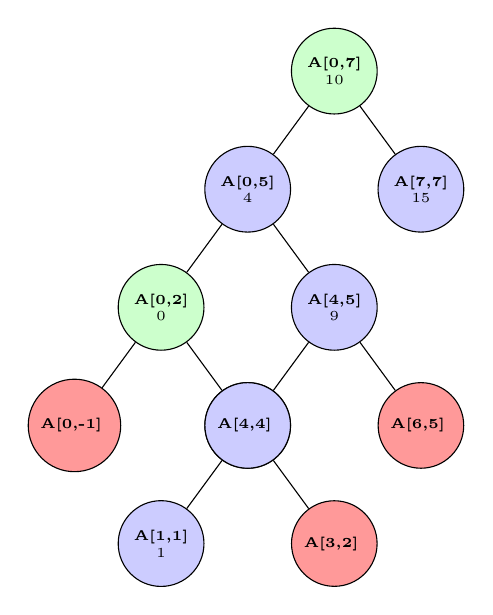
\begin{tikzpicture}[level distance=1.5cm, sibling distance=2.2cm, every node/.style={font=\tiny}]
          % Root node
          \node[circle, draw, fill=green!20, minimum size=1cm, align=center] (root) {
            \textbf{A[0,7]} \\
            10
          }
          % Left child
          child {node[circle, draw, fill=blue!20, minimum size=1cm, align=center] {
                  \textbf{A[0,5]} \\
                  4
                }
              % New children for this step
              child {node[circle, draw, fill=green!20, minimum size=1cm, align=center] {
                      \textbf{A[0,2]}\\
                      0
                    }
                  child {node[circle, draw, fill=red!40, minimum size=1cm, align=center] {
                          \textbf{A[0,-1]}
                        }}
                  child {node[circle, draw, fill=blue!20, minimum size=1cm, align=center] {
                          \textbf{A[1,2]}\\
                          3
                        }
                      child {node[circle, draw, fill=blue!20, minimum size=1cm, align=center] {
                              \textbf{A[1,1]}\\
                              1
                            }
                        }
                      child {node[circle, draw, fill=red!40, minimum size=1cm, align=center] {
                              \textbf{A[3,2]}
                            }
                        }
                    }
                }
              child {node[circle, draw, fill=blue!20, minimum size=1cm, align=center] {
                      \textbf{A[4,5]}\\
                      9
                    }
                  child {node[circle, draw, fill=blue!20, minimum size=1cm, align=center] {
                          \textbf{A[4,4]}
                        }}
                  child {node[circle, draw, fill=red!40, minimum size=1cm, align=center] {
                          \textbf{A[6,5]}
                        }}
                }
            }
          % Right child
          child {node[circle, draw, fill=blue!20, minimum size=1cm, align=center] {
                  \textbf{A[7,7]} \\
                  15
                }
            };
        \end{tikzpicture}
      \end{center}
    \end{minipage}
  \end{columns}
\end{frame}


% Step 5: Final sorted array
\begin{frame}{Randomized Quicksort: Final Sorted Array}
  The final sorted array is:
  \[
    \renewcommand{\arraystretch}{1.5}
    \begin{array}{|c|c|c|c|c|c|c|c|}
      \hline
      0 & 1 & 3 & 4 & 6 & 9 & 10 & 15 \\
      \hline
    \end{array}
  \]
\end{frame}

\begin{frame}[fragile]{Quicksort Implementation (Python)}
  \begin{lstlisting}
import random
def quicksort(arr):
    if len(arr) <= 1:
        return arr
    pivot_idx = random.randrange(len(arr))  # Random index
    pivot = arr[pivot_idx]
    left = [x for x in arr if x < pivot]
    middle = [x for x in arr if x == pivot]
    right = [x for x in arr if x > pivot]
    return quicksort(left) + middle + quicksort(right)
  \end{lstlisting}
\end{frame}